\documentclass[fleqn, a4paper, 12pt, twoside]{article}
\usepackage{exsheets}
\usepackage{amsmath, amssymb, amsthm} %standard AMS packages
\usepackage{mathtools}
\usepackage{marginnote} %marginnotes
\usepackage{gensymb} %miscellaneous symbols
\usepackage{commath} %differential symbols
\usepackage{xcolor} %colours
\usepackage{cancel} %cancelling terms
\usepackage{siunitx} %formatting units
\usepackage{tikz, pgfplots} %diagrams
	\usetikzlibrary{calc, hobby, patterns, intersections}
\usepackage{graphicx} %inserting graphics
\usepackage{hyperref} %hyperlinks
\usepackage{datetime} %date and time
\usepackage{ulem} %underline for \emph{}
\usepackage{xfrac} %inline fractions
\usepackage{enumerate} %numbered lists
\usepackage{float} %inserting floats
\usepackage[american voltages, american currents]{circuitikz} %circuit diagrams

\newcommand\numberthis{\addtocounter{equation}{1}\tag{\theequation}} %adds numbers to specific equations in non-numbered list of equations

\newcommand{\AxisRotator}[1][rotate=0]{
	\tikz [x=0.25cm,y=0.60cm,line width=.2ex,-stealth,#1] \draw (0,0) arc (-150:150:1 and 1);%
} %rotation symbols on axes

\theoremstyle{definition}
\newtheorem{example}{Example}
\newtheorem{definition}{Definition}

\theoremstyle{theorem}
\newtheorem{theorem}{Theorem}
\newtheorem{law}{Law}

\newcommand{\curl}{\mathrm{curl\,}}

\makeatletter
\@addtoreset{section}{part} %resets section numbers in new part
\makeatother

\newcommand{\partbreak}{\clearpage} %starts every part on a new page

\newcommand\blfootnote[1]{%
	\begingroup
	\renewcommand\thefootnote{}\footnote{#1}%
	\addtocounter{footnote}{-1}%
	\endgroup
}

\SetupExSheets{solution/print = true}

%opening
\title{Introduction to Electrical Engineering}
\author{Aakash Jog}
\date{2014-15}

\begin{document}

\maketitle
%\setlength{\mathindent}{0pt}

\blfootnote
{	
	\begin{figure}[H]
		
\includegraphics[height = 12pt]{cc.eps}
		\includegraphics[height = 12pt]{by.eps}
		\includegraphics[height = 12pt]{nc.eps}
		
\includegraphics[height = 12pt]{sa.eps}
	\end{figure}
	This work is licensed under the Creative Commons Attribution-NonCommercial-ShareAlike 4.0 International License. To view a copy of this license, visit \url{http://creativecommons.org/licenses/by-nc-sa/4.0/}.
} %CC-BY-NC-SA licencse

\tableofcontents

 \newpage
%\part{General Information}

\section{Lecturer Information}

\textbf{Prof. Moshe Tur}\\
~\\
Office: Wolfson 413\\
Telephone: 03-640-8125\\
E-mail: tur@post.tau.ac.il\\

\section{Required Reading}

C.A. Desoer and E.S. Kuh: \textit{Basic Circuit Theory}, Mc-Graw-Hill, International Edition.

\newpage
\part{Basic Definitions and Laws}

\section{Basic Definitions}

\begin{definition}[Electrical circuit]
	A collection of interconnected components.
\end{definition}

\begin{definition}[Lumped component]
	An electrical component whose dimensions are very very small compared to the wavelength of the electromagnetic waves passing through it is called a lumped component.
\end{definition}

\begin{definition}[One port device]
	An electrical component with two terminals is called a one port device.
	\begin{figure}[H]
		\begin{circuitikz}
			\draw (0,0) -- (1,0) to [generic] (2,0) -- (3,0);
		\end{circuitikz}
	\end{figure}
\end{definition}

\begin{definition}[Nodes and branches]
	In the figure, all the black dots are called nodes. The parts of the circuit between two nodes are called branches.
	\begin{figure}[H]
		\begin{circuitikz}[scale = 0.8]
			\draw (0,0) to [generic, *-*, i<=$i_2$] (5,5) to [generic, *-*, i<=$i_1$] (10,0);
			\draw (0,0) to [generic, *-*, i<=$i_3$] (10,0);
			\draw (0,0) to [generic, *-*, i<=$i_5$] (5,-5) to [generic, *-*, i>=$i_2$] (10,0);
		\end{circuitikz}
	\end{figure}
\end{definition}

\section{Kirchoff's Laws}

\subsection{Kirchoff's Current Law}

\begin{law}[Kirchoff's Current Law]\label{KCL}
	The sum of all currents entering or exiting a node is zero.
\end{law}
\begin{figure}[H]
	\begin{circuitikz}[scale = 0.8]
		\draw (0,0) to [generic, *-*, i<=$i_2$] (5,5) to [generic, *-*, i<=$i_1$] (10,0);
		\draw (0,0) to [generic, *-*, i<=$i_3$] (10,0);
		\draw (0,0) to [generic, *-*, i<=$i_5$] (5,-5) to [generic, *-*, i>=$i_2$] (10,0);
	\end{circuitikz}
\end{figure}
	
\begin{equation*}
	i_1 + i_3 - i_4 = 0
\end{equation*}

\subsection{Kirchoff's Voltage Law}

\begin{law}[Kirchoff's Voltage Law]\label{KVL}
	The sum of all branch voltages along a closed loop is zero.
\end{law}
\begin{figure}[H]
	\begin{circuitikz}[american voltages]
		\draw (0,0) to [generic = 1, v<=$v_1$] (0,5) to [generic = 2, v<=$v_2$] (0,10) -- (5,10) to [generic = 3, v<=$v_3$] (5,5) to [generic = 5, v>=$v_5$] (5,0) -- (0,0);
		\draw (0,5) to [generic = 4, v>=$v_4$] (5,5);
	\end{circuitikz}
\end{figure}

\begin{align*}
	v_1 - v_4 - v_5 &= 0\\
	v_2 + v_3 + v_4 &= 0\\
	v_1 + v_2 + v_3 - v_5 &= 0
\end{align*}

\section{Components}

\subsection{Resistors}

\begin{definition}[Resistor]
	A two terminal component is called a resistor if the voltage across it at any given time $t$ is a function of the current at the same time $t$.
\end{definition}

\subsubsection{Linear Time Independent Resistor}

\begin{figure}[H]
	\begin{circuitikz}[american voltages]
		\draw (0,0) to [R, v<=$v$, i>=$i$] (5,0);
	\end{circuitikz}
\end{figure}

\begin{figure}[H]
	\begin{tikzpicture}[scale = 0.5]
		\begin{scope}[stealth-stealth]
			\draw (-5,0) -- (5,0) node [right] {$i$};
			\draw (0,-5) -- (0,5) node [above] {$v$};
		\end{scope}
		
		\draw (-4,-4) -- (4,4);
	\end{tikzpicture}
\end{figure}

\begin{align*}
	v(t) &= R \cdot i(t)\\
	i(t) &= G \cdot v(t)
\end{align*}
$R$ is called the resistance and $G$ is called the conductance.

\subsubsection{Non-linear Resistors (Diodes)}

\begin{figure}[H]
	\begin{circuitikz}[american voltages]
		\draw (0,0) to [Do, v<=$v$, i>=$i$] (5,0);
	\end{circuitikz}
\end{figure}

\begin{align*}
	i(t) &= I_s \left( e^{\dfrac{q \cdot v(t)}{k T}} - 1 \right)
\end{align*}

\begin{align*}
	I_s &= \textnormal{reverse current}\\
	k &= \textnormal{Boltzman constant}\\
	T &= \textnormal{$a$bsolute temperature}\\
	q &= \textnormal{electronic change}\\
	\dfrac{k T}{q} &= 0.026 (\textnormal{ at } 300 \si{\kelvin})
\end{align*}

\begin{figure}[H]
	\begin{tikzpicture}[scale = 0.5]
		\def\reverseCurrent{-0.2};
	
		\begin{scope}[stealth-stealth]
			\draw (-5,0) -- (5,0) node [right] {$v$};
			\draw (0,-5) -- (0,5) node [above] {$i$};
		\end{scope}
			
		\draw (-4,\reverseCurrent) to [out = 0, in = 190] (0,0) to [out = 10, in = 260] (2,4);
	\end{tikzpicture}
\end{figure}

An ideal diode has a $i$-$v$ graph like
\begin{figure}[H]
	\begin{tikzpicture}[scale = 0.5]
		\begin{scope}[stealth-stealth, lightgray]
			\draw (-5,0) -- (5,0) node [right] {$v$};
			\draw (0,-5) -- (0,5) node [above] {$i$};
		\end{scope}
		
		\draw (-4,0) -- (0,0) -- (0,4);;
	\end{tikzpicture}
\end{figure}

\subsection{Independent Sources}

\subsubsection{Voltage Sources}

\begin{definition}[Voltage source]
	A two terminal component is called a voltage source if the voltage on its terminals is independent of the current through it.
	
	\begin{figure}[H]
		\begin{circuitikz}
			\draw (0,0) to [american voltage source, v = $v_s(t)$, i>=$i$] (0,5) to (5,5) to [generic] (5,0) to (0,0);
		\end{circuitikz}
	\end{figure}
	
	\begin{figure}[H]
		\begin{tikzpicture}[scale = 0.5]
			\def\i{2};
		
			\begin{scope}[stealth-stealth]
				\draw (-5,0) -- (5,0) node [right] {$i$};
				\draw (0,-5) -- (0,5) node [above] {$v$};
			\end{scope}
			
			\draw (-4,\i) -- (4,\i);
		\end{tikzpicture}
	\end{figure}
		
\end{definition}

\subsubsection{Current Sources}

\begin{definition}[Current source]
	A two terminal component is called a current source if it can supply a current $i_s(t)$ independent of the voltage across its terminals.

	\begin{figure}[H]
		\begin{circuitikz}
			\draw (0,0) to [american current source, i = $i_s(t)$] (0,5) to (5,5) to [generic] (5,0) to (0,0);
		\end{circuitikz}
	\end{figure}

	\begin{figure}[H]
		\begin{tikzpicture}[scale = 0.5]
			\def\v{2};
			
			\begin{scope}[stealth-stealth]
				\draw (-5,0) -- (5,0) node [right] {$i$};
				\draw (0,-5) -- (0,5) node [above] {$v$};
			\end{scope}
			
			\draw (\v,-4) -- (\v,4);
		\end{tikzpicture}
	\end{figure}
\end{definition}

\subsubsection{Real Batteries}

\begin{figure}[H]
	\begin{tikzpicture}[scale = 0.5]
		\def\v0{2};
		
		\begin{scope}[stealth-stealth]
			\draw (-5,0) -- (5,0) node [right] {$i$};
			\draw (0,-5) -- (0,5) node [above] {$v$};
		\end{scope}
		
		\draw (0,\v0) -- (2*\v0,0);
	\end{tikzpicture}
\end{figure}

\begin{figure}[H]
	\begin{circuitikz}
		\draw (0,0) to [battery1 = $V_0$] (0,2) to [R = $R_s$] (0,4) to (4,4) to [generic] (4,0) to (0,0);
	\end{circuitikz}
\end{figure}

\begin{align*}
	0 &= -V_0 + v_R + v\\
	v &= V_0 - v_R\\
	\therefore v &= V_0 - R_s i
\end{align*}

\subsection{Capacitor}

\begin{definition}[Capacitor]
	A capacitor is a two terminal device where $V$ is a fucntion of $q$.
	\begin{figure}[H]
		\begin{circuitikz}
			\draw (0,0) to [C] (5,0);
		\end{circuitikz}
	\end{figure}
\end{definition}

\subsubsection{Linear Capacitors}

If the charges on the terminals of a capacitor are $+q$ and $-q$, and the potential difference across it is $v$, the ratio between $q$ and $v$ is said to be the capacitance.\\
The unit of capacitance is farad or $\si{\farad}$.
\begin{align*}
	q &= C v\\
	\therefore i &= C \dod{v}{t}\\
	\therefore v(t) &= v(t_0) + \dfrac{1}{C} \int\limits_{t_0}^{t} i(t) \dif t
\end{align*}
\begin{figure}[H]
	\begin{circuitikz}
		\draw (0,0) to [C, v = $v$] (5,0);
	\end{circuitikz}
\end{figure}

\subsection{Inductor}

\begin{definition}[Inductor]
	\begin{figure}[H]
		\begin{circuitikz}
			\draw (0,0) to [L, v = $v(t)$, i> = $i(t)$] (5,0);
		\end{circuitikz}
	\end{figure}
	\begin{align*}
		v(t) &= \dod{\varphi}{t}\\
		\therefore v(t) &= L \dod{i}{t}\\
		\therefore i(t) &= i(t_0) + \dfrac{1}{L} \int\limits_{t_0}^{t} v(t) \dif t
	\end{align*}
\end{definition}

\section{Waveforms}

\subsection{DC (Constant Function)}

\begin{figure}[H]
	\begin{tikzpicture}[scale = 0.5]		
		\begin{scope}[stealth-stealth]
			\draw (-5,0) -- (5,0) node [right] {$t$};
			\draw (0,-5) -- (0,5);
		\end{scope}
		
		\draw (-4,3) -- (4,3);
		\end{tikzpicture}
\end{figure}

\subsection{Sinusoidal Wave}

\begin{figure}[H]
	\begin{tikzpicture}[scale = 0.5]		
		\begin{scope}[stealth-stealth]
			\draw (-5,0) -- (5,0) node [right] {$t$};
			\draw (0,-5) -- (0,5);
		\end{scope}
		
		\draw [domain = 0: 4] plot (\x, {(cos(2*\x r)});
	\end{tikzpicture}
\end{figure}

\subsection{Step Function}

\begin{figure}[H]
	\begin{tikzpicture}[scale = 0.5]	
		\begin{scope}[gray, stealth-stealth]
			\draw (-5,0) -- (5,0) node [right] {$t$};
			\draw (0,-5) -- (0,5);
		\end{scope}
		
		\draw (-4,0) -- (1,0) -- (1,2) -- (4,2);
		
		\node [below] at (1,0) {$\tau$};
	\end{tikzpicture}
\end{figure}

\begin{align*}
	u(t) &=
		\begin{cases}
			0 &;\quad t < 0\\
			\dfrac{1}{2} &;\quad t = \tau\\
			1 &;\quad t > \tau\\
		\end{cases}
\end{align*}

\subsection{Rectangular Pulse}

\begin{figure}[H]
	\begin{tikzpicture}[scale = 0.5]	
		\begin{scope}[gray, stealth-stealth]
			\draw (-5,0) -- (5,0) node [right] {$t$};
			\draw (0,-5) -- (0,5);
		\end{scope}
		
		\draw (-4,0) -- (0,0) -- (0,2) -- (2,2) -- (2,0) -- (4,0);
		
		\node [below] at (2,0) {$\Delta$};
	\end{tikzpicture}
\end{figure}

\begin{align*}
	P_{\Delta}(t) &= \dfrac{u(t) - u(t - \Delta)}{\Delta}
\end{align*}

\begin{align*}
	P_{\Delta}(t) &=
		\begin{cases}
			0 &;\quad t < 0\\
			\dfrac{1}{\Delta} &;\quad t = 0\\
			1 &;\quad t > 0\\
		\end{cases}
\end{align*}

\subsection{Dirac $\delta$ function}

\begin{align*}
	\delta(t) &= \lim\limits_{\Delta \to 0} P_{\Delta}(t)
\end{align*}

\begin{align*}
	S(\Delta) &= \int\limits_{-\infty}^{\infty} P_{\Delta}(t) f(t) \dif t\\
	\intertext{As $\Delta \to 0$,}
	S(\Delta) &= \int\limits_{-\infty}^{\infty} P_{\Delta}(t) f(0) \dif t\\
	&= f(0) \int\limits_{-\infty}^{\infty} P_0(t) \dif t\\
	&= f(0)
\end{align*}

\begin{align*}
	\delta(t) &=
		\begin{cases}
			0 &;\quad t \neq 0\\
			\infty &;\quad t = 0\\
		\end{cases}
\end{align*}

\begin{align*}
	\int\limits_{-\infty}^{\infty} \delta(t) f(t) \dif t &= f(0)\\
	\int\limits_{-\infty}^{\infty} \delta(t - \tau) f(t) \dif t &= f(\tau)\\
	\int\limits_{-\infty}^{\infty} \delta(a t) f(t) \dif t &= \dfrac{1}{|a|} \delta(t)
\end{align*}

\subsection{Ramp Function}

\begin{figure}[H]
	\begin{tikzpicture}[scale = 0.5]	
		\begin{scope}[gray, stealth-stealth]
			\draw (-5,0) -- (5,0) node [right] {$t$};
			\draw (0,-5) -- (0,5);
		\end{scope}
		
		\draw (-4,0) -- (0,0) -- (4,4);
	\end{tikzpicture}
\end{figure}

\begin{align*}
	r(t) &= t u(t)
\end{align*}

\subsection{Doublet Function}

\begin{align*}
	\delta' (t) &= \dod{\delta(t)}{t}
\end{align*}

\subsection{Relation Between Standard Waveforms}

\begin{equation*}
	r(t) \xrightleftharpoons[\int_{-\infty}^{t}]{\od{}{t}} u(t) \xrightleftharpoons[\int_{-\infty}^{t}]{\od{}{t}} \delta(t) \xrightleftharpoons[\int_{-\infty}^{t}]{\od{}{t}} \delta' (t) 
\end{equation*}

\begin{question}
	Express the following wave as a sum of standard waveforms.
	\begin{figure}[H]
		\begin{tikzpicture}
			\begin{scope}[gray, stealth-stealth]
				\draw (-1,0) -- (5,0) node [right] {$t$};
				\draw (0,-1) -- (0,5);
			\end{scope}
			
			\draw (0,0) -- (1,0) -- (1,1) -- (2,1) -- (2,2) -- (4,2);
			
			\foreach \i in {1,...,4}
			{
				\node [below] at (\i,0) {$\i$};
			}
		\end{tikzpicture}
	\end{figure}
\end{question}

\begin{solution}
	\begin{equation*}
		f(t) = u(t - 1) + u(t - 2)
	\end{equation*}
\end{solution}

\begin{question}
	Express the following wave as a sum of standard waveforms.
	\begin{figure}[H]
		\begin{tikzpicture}
			\begin{scope}[gray, stealth-stealth]
				\draw (-1,0) -- (5,0) node [right] {$t$};
				\draw (0,-1) -- (0,5);
			\end{scope}
			
			\draw (0,0) -- (1,1) -- (4,1);
			
			\foreach \i in {1,...,4}
			{
				\node [below] at (\i,0) {$\i$};
			}
		\end{tikzpicture}
	\end{figure}
\end{question}

\begin{solution}
	\begin{equation*}
		f(t) = r(t) + r(t - 1)
	\end{equation*}
\end{solution}

\section{Power and Energy}

The instantaneous power supplied to a load is
\begin{align*}
	P(t) &= v(t) \cdot i(t)
\end{align*}
where $v(t)$ and $i(t)$ are in matched directions.

The energy supplied to a load from time $t_0$ to time $t$ is
\begin{align*}
	W(t_0, t) &= \int\limits_{t_0}^{t} P(t) \dif t\\
	&= \int\limits_{t_0}^{t} v(t) \cdot i(t) \dif t
\end{align*}

\subsection{Energy Stored in a Capacitor}

\begin{align*}
	W(t_0, t) &= \int\limits_{t_0}^{t} v(t) i(t) \dif t\\
	\intertext{As $i(t) = \dod{q}{t}$, $\dif q = i(t) \dif t$. Therefore,}
	W(t_0, t) &= \int\limits_{q(t_0)}^{q(t)} v(q) \dif q\\
	&= \int\limits_{q(t_0)}^{q(t)} \dfrac{q}{C} \dif q\\
	&= \dfrac{q^2}{2c}\\
	&= \dfrac{1}{2} c v^2
\end{align*}

\subsection{Energy Stored in an Inductor}

\begin{align*}
	W(t_0, t) &= \int\limits_{t_0}^{t} v(t) i(t) \dif t\\
	\intertext{As $v(t) = \dod{\varphi}{t}$, $\dif \varphi = v(t) \dif t$. Therefore,}
	W(t_0, t) &= \int\limits_{\varphi(t_0)}^{\varphi(t)} i(\varphi) \dif \varphi\\
	&= \dfrac{\varphi^2}{2 L}\\
	&= \dfrac{1}{2} L i^2
\end{align*}

\newpage
\part{Simple Circuits}

\section{Equivalent Circuits}

\begin{definition}
	Two circuits are said to be equivalent if they have the same $v(t)$-$i(t)$ relationships.
\end{definition}

\begin{example}
	\begin{figure}[H]
		\begin{circuitikz}
			\draw (0,0) to [R = $R_1$] (2,0) to [R = $R_2$] (4,0); 
		\end{circuitikz}
	\end{figure}
	
	Let the voltage across $R_1$ be $v_1$ and across $R_2$ be $v_2$.\\
	Let the current through $R_1$ be $i_1$ and through $R_2$ be $i_2$.\\
	Therefore,
	\begin{align*}
		v_1 &= f_1(i_1)\\
		v_2 &= f_2(i_2)
	\end{align*}
	Therefore,
	\begin{align*}
		v &= v_1 + v_2\\
		&= f_1(i_1) + f_2(i_2)\\
		&= f_1(i) + f_2(i)\\
		&= f_3(i)
	\end{align*}
	Therefore, the system of resistors is equivalent to a single resistor $R_3$.
\end{example}

\subsection{Series Connections}

If circuit elements are connected in series, by \nameref{KCL}, the current passing through all of them is equal.
By \nameref{KVL}, the net potential difference is the sum of the voltages across each of them.

\subsubsection{Resistors in Series}

\begin{figure}[H]
	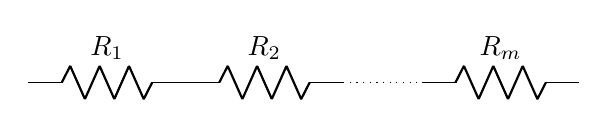
\begin{tikzpicture}
		\draw (0,0) to [R = $R_1$] (2,0) to [R = $R_2$] (4,0);
		\draw [dotted] (4,0) to (5,0);
		\draw (5,0) to [R = $R_m$] (7,0);
	\end{tikzpicture}
\end{figure}

\begin{align*}
	v &= \sum_{k = 1}^{m} v_k\\
	&= \sum_{k = 1}^{m} R_k i_k\\
	&= \sum_{k = 1}^{m} R_k i\\
	&= i \sum_{k = 1}^{m} R_k\\
	\therefore v &= R i\\
	\therefore R &= \sum_{k = 1}^{m} R_k
\end{align*}

\subsubsection{Voltage Sources in Series}

\begin{figure}[H]
	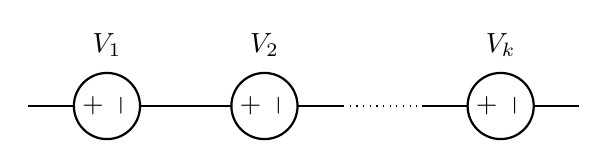
\begin{tikzpicture}
		\draw (0,0) to [V = $V_1$] (2,0) to [V = $V_2$] (4,0);
		\draw [dotted] (4,0) to (5,0);
		\draw (5,0) to [V = $V_k$] (7,0);
	\end{tikzpicture}
\end{figure}

By \nameref{KVL},
\begin{align*}
	v &= \sum_{k = 1}^{m} v_k
\end{align*}

\subsubsection{Half Wave Rectifier}

\begin{figure}[H]
	\begin{circuitikz}
		\draw (0,0) to (2,0) to [R = $R_1$, v = $v_1$] (2,-2) to [Do, v = $ $] (2,-4) to (0,-4) to [sV = $v$] (0,0);
	\end{circuitikz}
	\caption{Half Wave Rectifier}
\end{figure}

\begin{figure}[H]
	\begin{tikzpicture}
		\begin{scope}[stealth-stealth, lightgray]
			\draw (-5,0) -- (5,0) node [right] {$v$};
			\draw (0,-5) -- (0,5) node [above] {$i$};
		\end{scope}
		
		\begin{scope}
			\draw [red] (-4,0) -- (0,0) -- (0,4);
			\draw [blue] (-4,-4) -- (4,4);
		\end{scope}
	\end{tikzpicture}
\end{figure}

If the current flows in a direction such that the diode is in forward bias, it will allow the current to pass through.
If the current is in the opposite direction, it will provide infinite resistance.\\
Therefore, the wave representing the current in the circuit will be made up of only upper halves of the sine wave.

\begin{figure}[H]
	\begin{tikzpicture}
		\begin{scope}[stealth-stealth, lightgray]
			\draw (-5,0) -- (5,0) node [right] {$v$};
			\draw (0,-5) -- (0,5) node [above] {$i$};
		\end{scope}
		
		\begin{scope}[scale = 0.5]
			\draw [domain = 0:pi] plot (\x, {sin(\x r)});
			\draw (pi,0) -- (2*pi,0);
			\draw [domain = 2*pi:3*pi] plot (\x, {sin(\x r)});
		\end{scope}
	\end{tikzpicture}
\end{figure}

\subsubsection{Capacitors in Series}

\begin{align*}
	v_k(t) &= v_k(0) + \dfrac{1}{C_k} \int\limits_{0}^{t} i_k(t) \dif t\\
	v &= \sum_{k = 1}^{m} v_k(t)\\
	&= \sum_{k = 1}^{m} v_k(0) + \left( \sum_{k = 1}^{m} \dfrac{1}{C_k} \right) \int\limits_{0}^{t} i(t) \dif t\\
	\therefore v &= v(0) + \dfrac{1}{C} \int\limits_{0}^{t} i(t) \dif t\\
	\therefore \dfrac{1}{C} &= \sum_{k = 1}^{m} \dfrac{1}{C_k}
\end{align*}

\subsubsection{Inductors in Series}

\begin{figure}[H]
	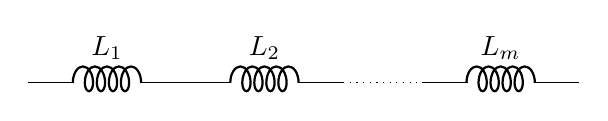
\begin{tikzpicture}
	\draw (0,0) to [L = $L_1$] (2,0) to [L = $L_2$] (4,0);
	\draw [dotted] (4,0) to (5,0);
	\draw (5,0) to [L = $L_m$] (7,0);
	\end{tikzpicture}
\end{figure}

\begin{align*}
	v &= \sum_{k = 1}^{m} v_k\\
	&= \sum_{k = 1}^{m} L_k \dod{i_k}{t}\\
	&= \sum_{k = 1}^{m} L_k \dod{i}{t}\\
	&= \dod{i}{t} \sum_{k = 1}^{m} L_k\\
	\therefore v &= L \dod{i}{t}\\
	\therefore L &= \sum_{k = 1}^{m} L_k
\end{align*}

\subsection{Parallel Connections}

\subsubsection{Resistors in Parallel}

\begin{figure}[H]
	\begin{circuitikz}
			\draw (0,0) to (1,0) to (2,1) to [R = $R_{1}$] (4,1) to (5,0) to (6,0);
			\node [above] at (3,0) {$\vdots$};
			\draw (0,0) to (1,0) to (2,-1) to [R = $R_{k}$] (4,-1) to (5,0) to (6,0);
	\end{circuitikz}
\end{figure}

\begin{align*}
	i &= \sum_{k = 1}^{m} i_k\\
	&= \sum_{k = 1}^{m} G_k v_k\\
	&= v \sum_{k = 1}^{m} G_k\\
	\therefore v &= G i\\
	\therefore G &= \sum_{k = 1}^{m} G_k\\
	\therefore \dfrac{1}{R} &= \sum_{k = 1}^{m} \dfrac{1}{R_k}
\end{align*}

\subsubsection{Capacitors in Parallel}

\begin{align*}
	i &= \sum_{k = 1}^{m} i_k\\
	&= \sum_{k = 1}^{m} C_k \dod{v_k}{t}\\
	&= \sum_{k = 1}^{m} C_k \dod{v}{t}\\
	&= \dod{v}{t} \sum_{k = 1}^{m} C_k\\
	\therefore i &= C \dod{v}{t}\\
	\therefore C &= \sum_{k = 1}^{m} C_k
\end{align*}

\subsubsection{Inductors in Parallel}

\begin{figure}[H]
	\begin{circuitikz}
		\draw (0,0) to (1,0) to (2,1) to [L = $L_{1}$] (4,1) to (5,0) to (6,0);
		\node [above] at (3,0) {$\vdots$};
		\draw (0,0) to (1,0) to (2,-1) to [L = $L_{k}$] (4,-1) to (5,0) to (6,0);
	\end{circuitikz}
\end{figure}

\begin{align*}
	i_k(t) &= i_k(0) + \dfrac{1}{L_k} \int\limits_{0}^(t) v_k(t) \dif t\\
	i &= \sum_{k = 1}^{m} i_k(t)\\
	&= \sum_{k = 1}^{m} i_k(0) + \sum_{k = 1}^{m} \left( \dfrac{1}{L_k} \int\limits_{0}^{t} v_k(t) \dif t \right)
	&= \sum_{k = 1}^{m} i_k(0) + \sum_{k = 1}^{m} \left( \dfrac{1}{L_k} \int\limits_{0}^{t} v(t) \dif t \right)\\
	&= \sum_{k = 1}^{m} i_k(0) + \left( \sum_{k = 1}^{m} \dfrac{1}{L_k} \right) \int\limits_{0}^{t} v(t) \dif t\\
	\therefore i &= i(0) + \dfrac{1}{L} \int\limits_{0}^{t} v(t) \dif t\\
	\therefore \dfrac{1}{L} &= \sum_{k = 1}^{m} \dfrac{1}{L_k}
\end{align*}

\begin{theorem}[Th\'{e}venin - Norton Theorem]
	Let $\pi$ be a linear network connected by two terminals to an arbitrary load. $\pi$ comprises of independent sources, linear resistors, linear capacitors and linear inductors. These components may be time dependent. Let $\pi_0$ be the network derived from $\pi$ by zeroing all independent sources(A short is inserted in place of a voltage source, and a break is inserted in place of a current source). Let $e_{\textnormal{OC}}$ be the voltage of the open circuit $\pi$, i.e. without the load, between $1$ and $1'$. Let $i_{\textnormal{SC}}$ be the short circuit current flowing from $1$ to $1'$. Under these conditions for an arbitrary load, the voltage $v$ between $1$ and $1'$ and the current $i$ between $1$ and $1'$ through the load will not change if the network $\pi$ is replaced by the equivalent circuit of either Th\'{e}venin or Norton.
	\begin{figure}[H]
		\begin{tikzpicture}
			\coordinate (1) at (4,0);
			\coordinate (1') at (4,-4);
			
			\draw (0,0) -- (1) to [generic = load, v = $v$] (1') -- (0,-4) to [generic = $\pi$] (0,0);
		\end{tikzpicture}
	\end{figure}
	\begin{figure}[H]
		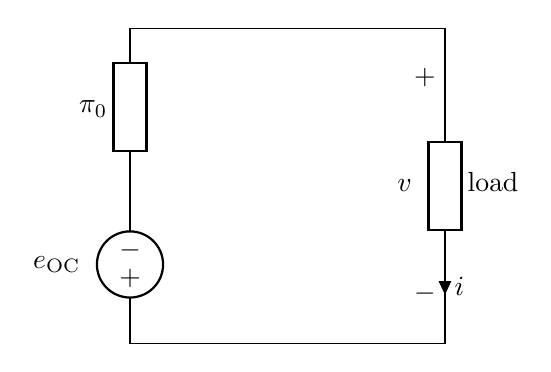
\begin{tikzpicture}
			\coordinate (1) at (4,0);
			\coordinate (1') at (4,-4);
			
			\draw (0,0) -- (1) to [generic = load, v = $v$, i = $i$] (1') -- (0,-4) to [V = $e_{\textnormal{OC}}$] (0,-2) to [generic = $\pi_0$] (0,0);
		\end{tikzpicture}
		\caption{Th\'{e}venin Equivalent Circuit}
	\end{figure}
	\begin{figure}[H]
		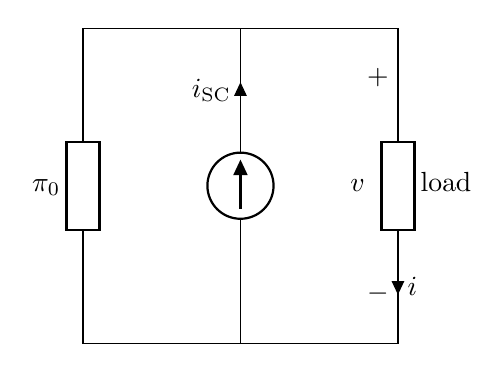
\begin{tikzpicture}
			\coordinate (1) at (4,0);
			\coordinate (1') at (4,-4);
			
			\draw (0,0) -- (1) to [generic = load, v = $v$, i = $i$] (1') -- (0,-4) to [generic = $\pi_0$] (0,0);
			
			\draw (2,-4) to [I = $i_{\textnormal{SC}}$] (2,0);
		\end{tikzpicture}
		\caption{Norton Equivalent Circuit}
	\end{figure}
\end{theorem}

\begin{question}
	\begin{figure}[H]
		\begin{circuitikz}
			\coordinate (1) at (2,2);
			\coordinate (1') at (2,0);
			
			\draw (0,0) to [V = $10 \si{\volt}$] (0,2) to [R = $5 \si{\ohm}$] (2,2) to [R = $5 \si{\ohm}$] (4,2);
			\draw (4,0) to [V= $20 \si{\volt}$] (4,2);
			\draw (0,0) -- (4,0);
			\draw (1) to [generic] (1');
		\end{circuitikz}
	\end{figure}
	\begin{figure}[H]
		\begin{circuitikz}
			\coordinate (1) at (2,2);
			\coordinate (1') at (2,0);
			
			\draw (0,0) to (0,2) to [R = $5 \si{\ohm}$] (2,2) to [R = $5 \si{\ohm}$] (4,2);
			\draw (4,0) to (4,2);
			\draw (0,0) -- (4,0);
			\draw (1) -- ++(90:1);
			\draw (1') -- ++(-90:1);
		\end{circuitikz}
	\end{figure}
\end{question}

\end{document}
